After acquiring, filtering and comparing the data, it has to be reported. The following chapter will show the reporting of the results of performance regression testing. It will touch on visualization and dectection of the performance regressions. \newline
\newline
As mentioned in Chapter 2, the choice of performance metric is very important. When making a report, this is what it will be based around. A report based on CPU time will have a different structure than a report based on bandwidth. The performance metrics require additional data to be able to show regressions. This additional data can be number of times the performance regression test has been executed or the number of times a particular function has been called. This kind of data can be usefull to determine if a performance regression has occured. If due to a new functionality a function is expected to be called twice as much since the last revision, a increase in performance can be expected.\newline

\section{Visualization}
When a report is created, a large amount of data can be usefull. Only it is very hard and error sensitive to look over those numbers. Visualization can be used to show the data in a way that might be easier to comprehend. By using visual representations such as a graph, can be used to spot a change in revisions. Just like the different structure for reports there are also different means to visualize results of performance regression testing.\newline
Transaction response time is the total time to process the request using the various
system resources \cite{jain2008art}. The transaction profile represents the lower bound value of the transaction response time for that transaction, or in other words, it is the
transaction response time when the transaction is the only one in the system (no queueing) \cite{ghaith2015anomaly}.\newline
The transaction profile can be visualised with a bar graph. By comparing the bar graphs of two revisions of the software, it is possible to detect the regressions.

\begin{figure}[h]
\begin{center}
  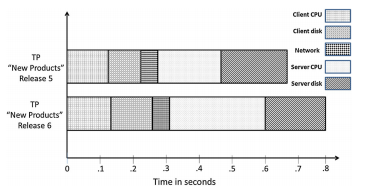
\includegraphics[width=0.5\textwidth]{Figures/TP.png}
\end{center}
  \caption{from ``Anomaly detection in performance regression testing by transaction profile estimation''\cite{ghaith2015anomaly}}

\end{figure}

The performance regression tests can also be represented in a normal graph. In a this graph a lot of revision can be visualized. This way there is a better overview of the performance regressions from the entire project and not just from two particular revisions. The following graph shows the number of written bytes for each revision.

\begin{figure}[h]
\begin{center}
  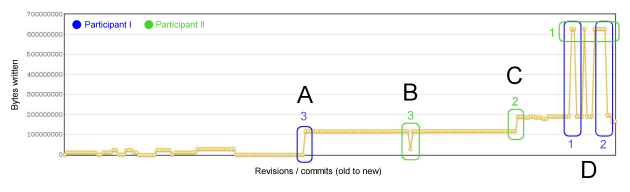
\includegraphics[width=0.5\textwidth]{Figures/bytegraph.png}
\end{center}
  \caption{from ``Detecting and analyzing I/O performance regressions''\cite{bezemer2014detecting}}

\end{figure}

These were only two of the many possibilties to visualize results of performance regression testing.

\section{Detection of performance regressions}
When a report and/or a visualization is created the regressions have to be detected. Detecting regressions is done by analyzing the report and finding a spike in performance. A spike in performance does not always mean there is a regression. It is possible that new functionality is added, which can cause a spike in performance. Looking at the figure above a spike in performance can be seen indicated with an ``A''. ``Phenomenon A: The increase was caused by a bugfix. Before this bugfix, data was not committed to the database''\cite{bezemer2014detecting}.\newline


\begin{figure}[h]
\begin{center}
  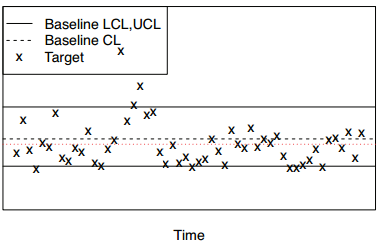
\includegraphics[scale=0.7]{Figures/controlchart.png}
\end{center}
  \caption{from ``Example of a control chart''\cite{nguyen2012using}}

\end{figure}




%mogelijk report techniek: transaction profile
%http://onlinelibrary.wiley.com/doi/10.1002/stvr.1573/pdf
%average precision and recall
%http://sail.cs.queensu.ca/publications/pubs/qsic2010_foo.pdf
